\documentclass[a4paper,12pt]{book} %\documentclass[a4paper,12pt]{scrbook}
%\usepackage{mathpazo}
\usepackage{amsmath} % จะใช้ package ของ math อื่นใด ให้เรียกก่อน fontspec
\usepackage{amssymb} % จะใช้ package ของ math อื่นใด ให้เรียกก่อน fontspec
\usepackage{amsfonts} % จะใช้ package ของ math อื่นใด ให้เรียกก่อน fontspec
\usepackage{mathspec} % เรียกใช้แค่นี้มีค่า = \usepackage[no-math]{fontspec}\usepackage{mathspec}
\usepackage{xunicode,xltxtra}
\XeTeXlinebreaklocale "th"
\XeTeXlinebreakskip = 0pt plus 1pt %
\defaultfontfeatures{Scale=1.23}
\renewcommand{\baselinestretch}{1.2}
\setmainfont{TH Sarabun New}
\newfontfamily\kodchasal{TH Kodchasal} % ตั้งชื่อฟอนต์ใหม่เพื่อให้ง่ายต่อการใช้งาน เผื่อว่าในเอกสารต้องการให้มีหลายฟอนต์ เวลาใช้ก็ {\examplefont ข้อความต่าง ๆ}
\newfontfamily\niramit{TH Niramit AS}
\usepackage{xcolor}
\definecolor{MyColor}{rgb}{0.3,0.4,0.5} % กำหนดสี และชื่อที่จะใช้เรียกสีโดย xcolor
\everymath{\displaystyle} % บังคับให้ทุกสมการเป็น displaystyle
\usepackage{tabls}
\usepackage{graphicx}
\usepackage{tabularx}
\usepackage{booktabs}
\usepackage{longtable}
\usepackage{wrapfig} %ตัวหนังสือล้อมรอบรูปหรือตารางได้ (wrapfigure,wraptable) *** ไม่สามารถอยู่ในพวก enumerate ได้
\usepackage[Glenn]{fncychap}
\usepackage{sectsty,ulem}
\allsectionsfont{\ulemheading{\uline}}
\makeatletter
\def\@seccntformat#1{\csname the#1\endcsname)\quad}
\makeatother
\usepackage{cellspace}
\usepackage[usenames,dvipsnames]{pstricks} 
\usepackage{epsfig} 
\usepackage{pst-grad} % For gradients
\usepackage{pst-plot} % For axes 
\usepackage{makecell}
\usepackage{fancyhdr}
\usepackage{lastpage}
\usepackage{fancybox}
\usepackage{multirow}
\usepackage{calc}
% ระยะช่องว่างหน้า+หลังเลขหรืออักษรในสมการ หน่วยเป็น mmu , 1 mmu = 1mu/1000 , 18mu = 1 em ,default = 500 mmu = 1/36 em 
% ตัวไหนจะให้มีระยะพิเศษก็ใส่ " นำหน้า เช่น $ x^{"2} หรือใส่ทีละคำให้ใส่เป็น $ x^{\"3yz"} $
% \setminwhitespace[XXXX] 
\setminwhitespace[3000] 

% เลือก Math Font ต่าง ๆ นา ๆ
%\setmathsfont(Digits,Latin){Asana Math}
%\setmathsfont(Digits,Latin){jsMath-cmr10}
%\setmathsfont(Digits,Latin){Kerkis}
%\setmathsfont(Digits,Latin){Neo Euler}
%\setmathsfont(Digits,Latin){Fontin}
%\setmathsfont(Digits,Latin){Plakken}
%\setmathsfont(Digits,Latin){DejaVu Serif}
%\setmathsfont(Digits,Latin){STIXGeneral}
%\setmathsfont(Digits,Latin){CMU Bright}
%\setmathsfont(Digits,Latin){Iwona Light}
%\setmathsfont(Digits,Latin,Greek)[Numbers={Lining,Proportional}]{Iwona Light}
%\setmathsfont(Digits,Latin,Greek){TH Sarabun New}
%\setmathsfont(Digits,Latin,Greek){Mathmos Original}
% ใช้ฟอนต์ OTF ในเอกสารแต่ MATH ใช้ฟอนต์ Math
%\usepackage[no-math]{fontspec}

% ใช้ฟอนต์ OTF ในเอกสารและ MATH ใช้ฟอนต์ OTF
%\usepackage[no-math]{fontspec}
%\usepackage{mathspec}
%\setmainfont{TH Sarabun New}
%\setallmainfonts(Digits,Latin,Greek){TH Sarabun New}
\setallmainfonts(Digits,Latin,Greek){TH Sarabun New}

% \setmathrm จะเปลี่ยนฟอนต์เฉพาะที่อยู่ในคำสั่ง \mathrm{.....} เท่านั้น
%\setmathrm{TH Sarabun New}
%\setmathsfont(Digits,Latin,Greek){TH Sarabun New}
%\setmathfont(Digits,Latin,Greek){TH Sarabun New}

%\AddToShipoutPictureFG{%
\begin{tikzpicture}[remember picture,overlay]
    \foreach \y in {0.5,1,1.5,2,2.5,3,3.5,...,29.5}{\draw[help lines] (0,\y) -- (21,\y);}
    \foreach \x in {0.5,1,1.5,2,2.5,3,3.5,...,21}{\draw[help lines] (\x,29.5) -- (\x,0);}
\end{tikzpicture}}
% -------------------------------- End Grid --------------------------------------


% ---------- เลขหน้าที่ขอบขวา -------------------------------------
\AddToShipoutPicture{%
\begin{tikzpicture}[remember picture,overlay]
	\checkoddpage
	\ifthenelse{\boolean{oddpage}}
	%{\node [xshift=20.5cm,yshift=5cm]  at (current page.west) [text width=1cm,fill=OliveDrab] {\color{white}\textbf{\thepage}};}
	%{\node [xshift=0.5cm,yshift=5cm]  at (current page.west) [align=right,text width=1cm,fill=OliveDrab] {\color{white}\textbf{\thepage}};}
	{\node [anchor=east,yshift=5cm]  at (current page.east) [text width=1.5cm,fill=OliveDrab] {\color{white}\codeB\large\textbf{\thepage}};}
	{\node [anchor=west,yshift=5cm]  at (current page.west) [align=right,text width=1.5cm,fill=OliveDrab] {\color{white}\codeB\large\textbf{\thepage}};}
\end{tikzpicture} }
% ----------จบ  เลขหน้าที่ขอบขวา ----------------------------------


% ------------------------ แถบด้านล่าง -----------------------------------------------
\AddToShipoutPictureBG{%
\begin{tikzpicture}[remember picture,overlay]
	\node at (current page.south west)
		{\begin{tikzpicture}[remember picture, overlay]
			\filldraw [draw=OldLace,fill=OldLace] (0,0) rectangle (\paperwidth,4cm);
		 \end{tikzpicture}
		};
\end{tikzpicture} }
% ------------------------ จบ  แถบด้านล่าง ------------------------------------------

% -------------------------------  Chapter Style --------------------
\usepackage[explicit]{titlesec}
\newcommand*\chapterlabel{}
\titleformat{\chapter}
	{\gdef\chapterlabel{}
		\normalfont\HUGE}
	%{\gdef\chapterlabel{\thechapter\ }}{0pt} 				% --- มีเลขบท ---
	{\gdef\chapterlabel{\phantom{}}}{0pt} 					% --- เอาเลขบทออก ทำเลขบทเอง ---
	{\begin{tikzpicture}[remember picture,overlay]
		\node[yshift=-3cm] at (current page.north west)
		{\begin{tikzpicture}[remember picture, overlay]
			%\draw[fill=LightSkyBlue] (0,0) rectangle (\paperwidth,3cm);
			%\draw [thick,postaction={decorate,decoration={text along path,text align=center,text={|\blanch\Huge\CHshift|CHAPTER }}}] (3,-1) -- (3,1);
			\draw [line width=2mm] (4.5,-2.2) -- (4.5,2.2) node[sloped,midway,above=-.2cm,font=\fontsize{52}{58}\blanch]{{\color{red}C}HAPTER};
			\draw [line width=2mm] (4.4,-2.2) -- (17,-2.2);
			%\node [xshift=.4\paperwidth,font=\fontsize{100}{108}] {\sig\color{black!10} \thechapter};
			\node [font=\fontsize{100}{108}] at (10.5,0) {\sig\color{black!10} \thechapter}; 
			%\draw (2.5,-1) node[rotate=90,font=\fontsize{52}{58}\blanch]{CHAPTER};
			%\node [anchor=east,xshift=.9\paperwidth,rectangle, rounded corners=20pt,inner sep=11pt, fill=red!20] {\akhanake\color{white}\chapterlabel#1};
			%\node [xshift=.6\paperwidth] {\akhanake\color{red}\chapterlabel#1};
			\node  at (10.5,0) {\quark\textbf{\color{DarkSlateGray}\chapterlabel#1}}; % quark = ชื่อฟอนต์ กำหนดเองใน premble
		\end{tikzpicture}
		};
	\end{tikzpicture}
	\thispagestyle{empty}		% ----- เอาเลขหน้าออกจากหน้าที่มี Chapter --------------
}
%\titlespacing*{\chapter}{0pt}{50pt}{-60pt}
\titlespacing*{\chapter}{0pt}{0pt}{0cm} % คุมช่องว่างระหว่างระหว่าง chapter กับ section 
% ------------------------ End Chapter Style -----------------------------------------------------

% ------------------------- หัวกระดาษ -----------------------------------------------------------------------------------------
\pagestyle{fancy}
\fancyhf{} % -- Clear Header & Footer ที่เป็นค่า Default ของ fancyhdr
\renewcommand{\headrulewidth}{0pt} % เอาเส้นที่ Header ออก
\newcommand{\BookHeadEven}{
	\tikz{ 
		\node[anchor=south west,fill=red!20, minimum height=2.9cm, minimum width=1cm, align=center] at (0,0)	{\color{white}\droid {\Huge{\textbf{\thechapter}}}};
		\draw[line width=2pt,color=red!20] (0,0) -- (14.6,0);
		\node[anchor=south east] at (14.6,0) {\color{DarkSlateGray}\huge{\textbf{www.pec9.com}}};
	}}
\newcommand{\BookHeadOdd}{
	\tikz{ 
		\draw[line width=2pt,color=red!20] (0,0) -- (14.6,0);
		\node[anchor=south east,fill=red!20, minimum height=2.9cm, minimum width=1cm, align=center] at (14.6,0)	{\color{white}\droid {\Huge{\textbf{\thechapter}}}};
		\node[anchor=south west] at (0,0) {\color{DarkSlateGray}\huge{\textbf{ติวสบาย ฟิสิกส์}}};
	}}
\usepackage[absolute]{textpos}
    \setlength{\TPHorizModule}{10mm}% 1 generic horizontal unit is equivalent to 10mm
    \setlength{\TPVertModule}{10mm}% 1 generic vertical unit is equivalent to 10mm
    \textblockorigin{0mm}{0mm}% top left corner set as origin
\fancyfoot[LO]{
	\begin{textblock}{1}(2.54,0)
		\BookHeadOdd
	\end{textblock}}
\fancyfoot[RE]{
	\begin{textblock}{1}(3.8,0)
		\BookHeadEven
	\end{textblock}}
%------------------------- จบหัวกระดาษ -----------------------------------------------------------------------------------------

%\renewcommand{\chaptername}{บทที่}
%\pagestyle{empty}
%\renewcommand{\labelenumi}{\roman{enumi}} % level 1 เป็นเลขโรมัน
%\setlist[enumerate,1]{leftmargin=*,resume} % ตั้งให้ enumerate level 1 ไม่ indent และต่อข้ออัตโนมัติ โดยไม่ต้องใช้ counter
%\newcommand*\circled[1]{ \tikz[baseline=(C.base)]\node[draw,circle,inner sep=1.2pt,line width=0.2mm,](C) {#1};}


% -------------------------- ADD QR CODE ------------------------------------------------------------------
\newcommand{\AddQR}[1]{
	\begin{tikzpicture}[remember picture,overlay]
		\node [xshift=10.5cm,yshift=2cm] at (current page.south west) {\includegraphics{qr_page#1.pdf}};
	\end{tikzpicture}
}

\AddToShipoutPictureFG{
	\ifthenelse{\value{page}=1}
	{
		\AddQR{1}
	}
	{
		\ifthenelse{\value{page}=2}
		{
			\AddQR{2}
		}
		{
			\ifthenelse{\value{page}=3}
			{
				\AddQR{3}
			}
			{
				\ifthenelse{\value{page}=4}
				{
					\AddQR{4}
				}
				{
				}
			}
		}
	}
}
% -------------------------------- End QR CODE ------------------------------------------

\begin{document}
\mainmatter % สำหรับ book


\chapter{การเคลื่อนที่}
	\section{การเคลื่อนที่แนวตรง}
		\begin{c3}\input{content-1.tex}\end{c3}
		\begin{enumerate}
\item    \begin{ljrp}\runningj 
            ระยะทางและการกระจัดของการเคลื่อนที่ต่อไปนี้ มีขนาดเท่ากับกี่เมตรตามลําดับ 
            \begin{4c}
                {12,8}{8,10}{8,12}{10,8}
            \end{4c}
        \end{ljrp}
        \begin{rp}{pic-jote-1.eps}\end{rp}
\end{enumerate}

	\section{การเคลื่อนที่แบบโปรเจกไทล์}
		\begin{c3}\begin{wrapfigure}{r}{0.5\textwidth}
  \vspace{-20pt}
  \begin{center}
    \includegraphics[width=0.4\textwidth]{content-8.eps}
  \end{center}
  \vspace{-20pt}
  \vspace{-10pt}
\end{wrapfigure}
\textbf{การเคลื่อนที่แบบโพรเจกไทล์}  คือ การเคลื่อนที่ในแนวโค้งรูปพาราโบลา  เกิดจากการเคลื่อนที่หลายมิติผสมกัน  ตัวอย่างเช่นหากเราขว้างวัตถุออกไปในแนวระดับจากดาดฟ้าตึกแห่งหนึ่ง  เราจะพบว่าวัตถุจะมีความพยายามที่จะเคลื่อนที่ไปในแนวระดับ (แกน X) ตามแรงที่เราขว้าง  พร้อมกันนั้นวัตถุจะถูกแรงโน้มถ่วงของโลก  ดึงให้เคลื่อนที่ตกลงมาในแนวดิ่ง (แกน Y) ด้วย    และเนื่องจากการเคลื่อนที่ทั้งสองแนวนี้เกิดในเวลาเดียวกัน      จึงเกิดการผสมผสานกันกลายเป็นการเคลื่อนที่แบบเส้นโค้งพาราโบลาพุ่งออกมาระหว่างกลางแนวระดับ (แกน X)  และแนวดิ่ง (แกน Y) ดังรูป  การเคลื่อนที่ในวิถีโค้งแบบนี้เรียกว่าเป็น \textbf{การเคลื่อนที่แบบโพรเจกไทล์}
\end{c3}
		\begin{enumerate}
\item \runningj \nonet ข้อใดใกล้เคียงกับการเคลื่อนที่แบบโพรเจกไทล์มากที่สุด
\begin{2c}
	{เครื่องบินขณะบินขึ้นจากสนามบิน}{เด็กเล่นไม้ลื่น}
	{ลูกเทนนิสที่ถูกตีออกไปข้างหน้า}{เครื่องร่อนขณะร่อนลง}
\end{2c}
\end{enumerate}

			\vspace{1in}
		\begin{enumerate}
	\item \runningj \nonet ยิงลูกปืนออกไปในแนวระดับทําให้ลูกปืนเคลื่อนที่แบบโพรเจกไทล์   ตอนที่ลูกปืนกําลังจะกระทบพื้น  ข้อใด\textbf{ถูกต้องที่สุด}   (ไม่ต้องคิดแรงต้านอากาศ)
	\begin{1c}
		{ความเร็วในแนวระดับเป็นศูนย์}
		{ความเร็วในแนวระดับมีขนาดมากกว่าตอนที่ถูกยิงออกมา }
		{ความเร็วในแนวระดับมีขนาดน้อยกว่าตอนที่ถูกยิงออกมาแต่ไม่เป็นศูนย์}
		{ความเร็วในแนวระดับเท่ากับความเร็วตอนต้นที่ลูกปืนถูกยิงออกมา}
	\end{1c}
\end{enumerate}

			\vfill
		\newpage
\chapter{สนามของแรง}
	\section{สนามแม่เหล็ก}
		\begin{c3}\subsection{สนามแม่เหล็กและเส้นสนามแม่เหล็ก}
\begin{minipage}{.5\textwidth}
\textbf{แม่เหล็ก (magnet)}  คือวัตถุที่ดูดเหล็กได้ และวัตถุที่แม่เหล็กส่งแรงกระทำเรียกว่า {\color{red} สารแม่เหล็ก (magnetic  substance)} 
\\\\
แท่งแม่เหล็ก 1 แท่งจะมี  2  ขั้วคือ \hfill ขั้วเหนือและ \\ ขั้วใต้ ขั้วแม่เหล็กชนิดเดียวกันจะผลักกันและขั้วต่างกันจะดูดกันเสมอ
\end{minipage} \hfill
\begin{adjustbox}{valign=c} 
    \begin{minipage}[c]{.45\linewidth}
        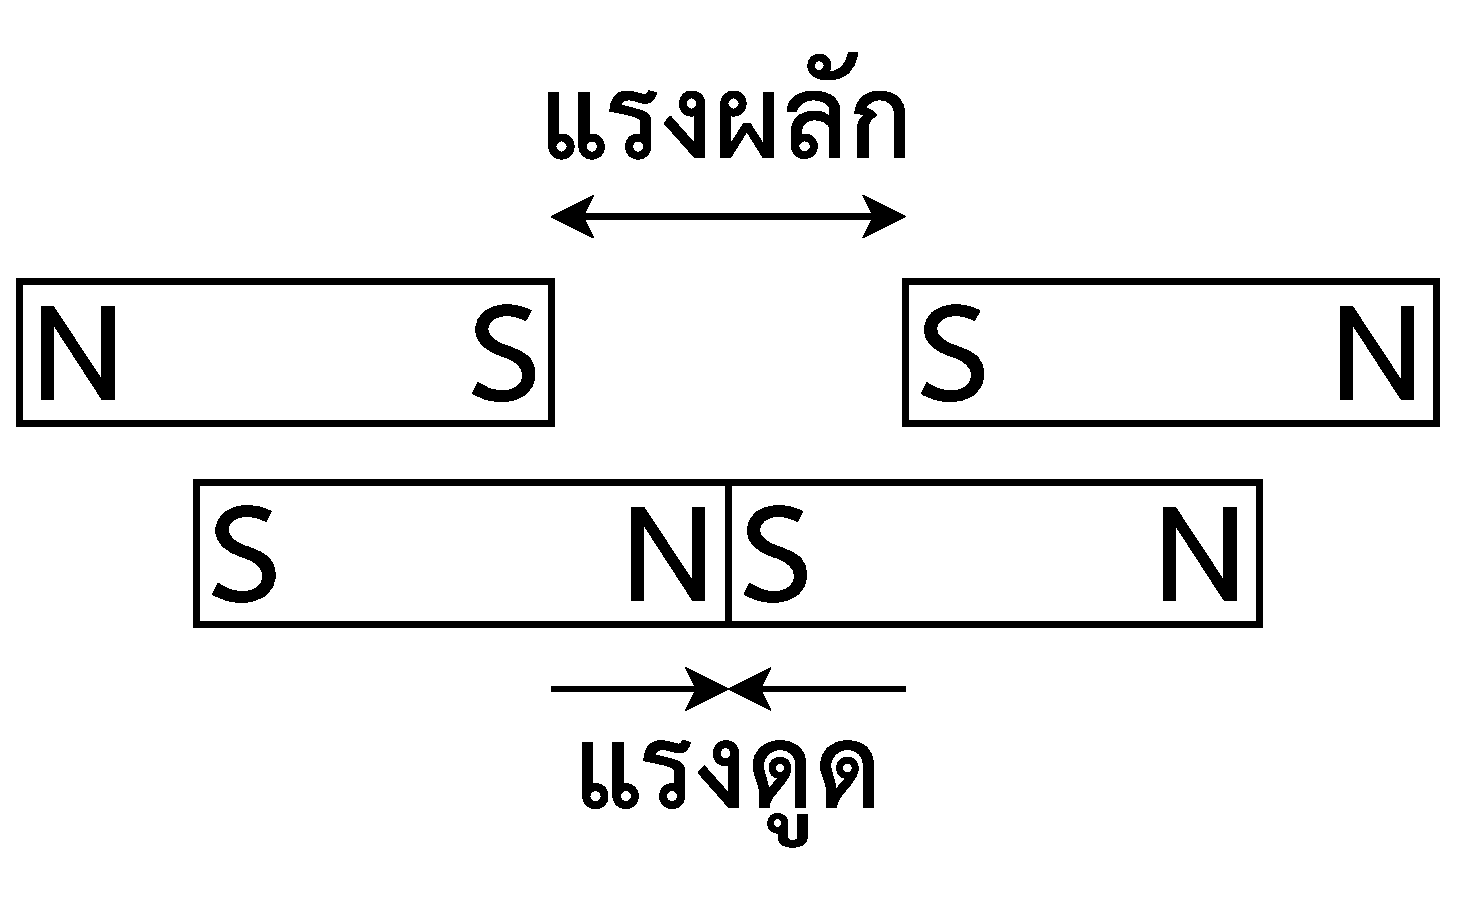
\includegraphics[width=\linewidth]{lesson2-1-1.eps}
    \end{minipage}
\end{adjustbox}

\tcblower

\begin{minipage}{.5\textwidth}
เมื่อวางแท่งแม่เหล็กลงบนแผ่นกระดาษ  แล้วโปรยผงเหล็กลงไป  จะพบว่า  แท่งแม่เหล็ก \hfill จะมีแรงกระทำต่อผงเหล็กเหล่านั้น  บริเวณที่มีแรงกระทำต่อผงเหล็กเรียกว่า \hfill {\color{red} สนามแม่เหล็ก (magnetic  field)}  \hfill      และแรงกระทำนี้จะทำให้ผงเหล็กเรียงตัวเป็นแนวเรียกแนวนี้ว่า {\color{red} \hfill เส้นสนามแม่เหล็ก  (magnetic  field  line)}
\end{minipage} \hfill
\begin{adjustbox}{valign=c} 
    \begin{minipage}[c]{.45\linewidth}
        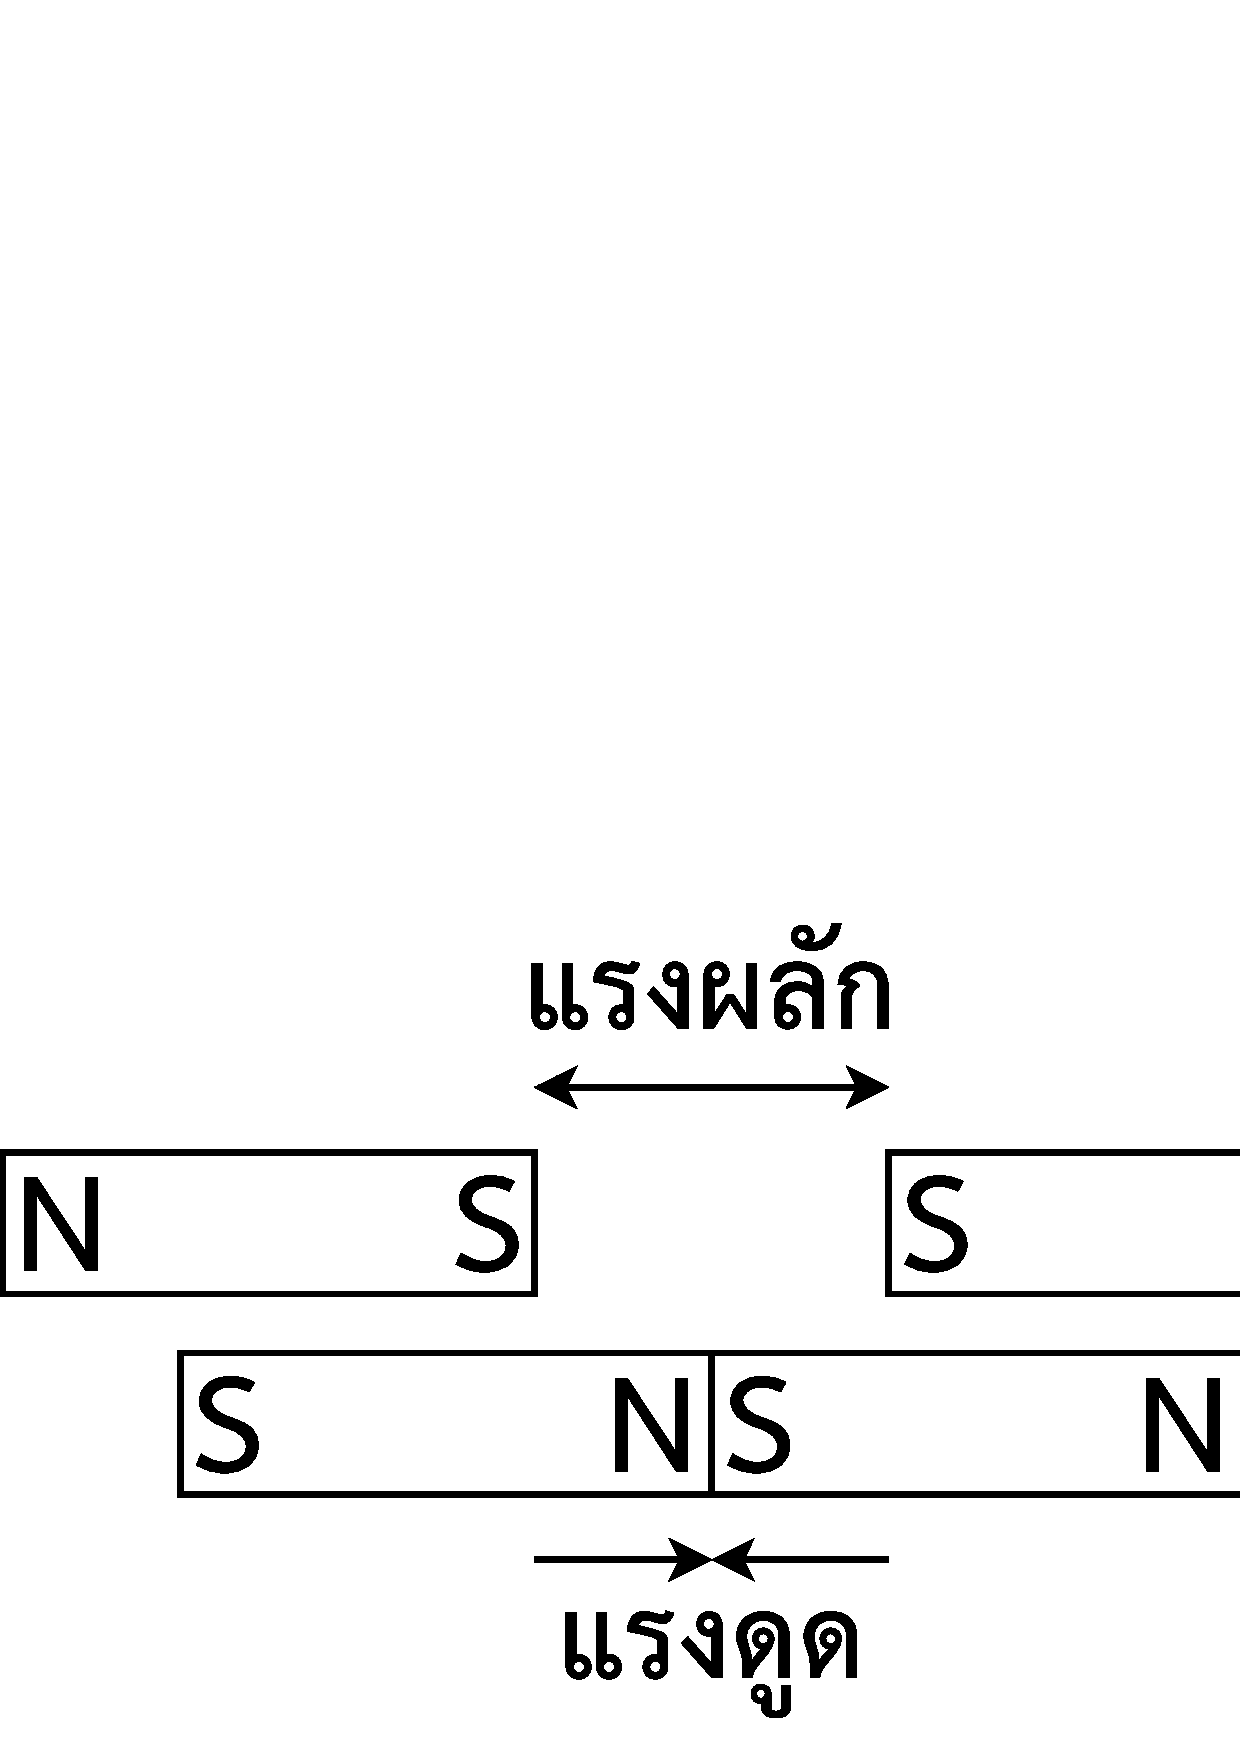
\includegraphics[width=\linewidth]{lesson2-1-1.jpg}
    \end{minipage}
\end{adjustbox}
\end{c3}
			\vfill
		\begin{enumerate}
\item   \begin{ljrp2}\runningj \nonet 
            จากแผนภาพแสดงลักษณะของเส้นสนาม
แม่เหล็กที่เกิดจากแท่งแม่เหล็กสองแท่ง   ข้อใดต่อไป
นี้เป็นขั้วแม่เหล็กเหนือ
            \begin{1c}
                {A และ C}{A และ D}{B และ C}{B และ D}
            \end{1c}
        \end{ljrp2}
        \begin{rp2}{l2j-1.eps}\end{rp2}
\end{enumerate}

			\vspace{1in}
		\begin{enumerate}
\item 	\begin{ljrp}\runningj \nonet โดยปกติเข็มทิศจะวางตัวตามแนวทิศเหนือ - ใต้  เมื่อนำเข็มมาวางใกล้ ๆ กับกึ่งกลางแท่งแม่เหล็กที่ตำแหน่งดังรูป  เข็มทิศจะชี้ในลักษณะใด
    \begin{2c}
        {\begin{adjustbox}{valign=t}\includegraphics[width=2cm]{l2j-2-2.eps}\end{adjustbox}}
        {\begin{adjustbox}{valign=t}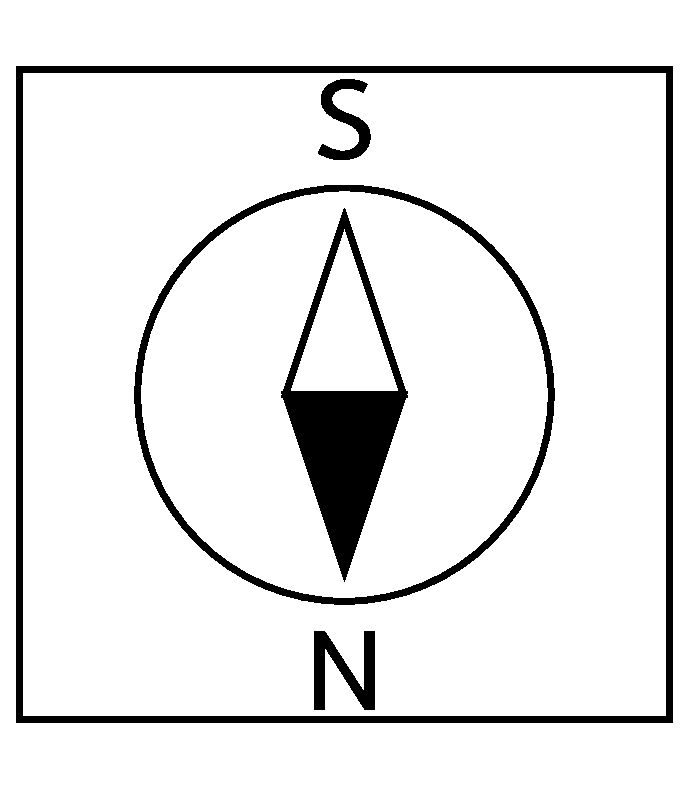
\includegraphics[width=2cm]{l2j-2-3.eps}\end{adjustbox}}
        {\begin{adjustbox}{valign=t}\includegraphics[width=2cm]{l2j-2-4.eps}\end{adjustbox}}
        {\begin{adjustbox}{valign=t}\includegraphics[width=2cm]{l2j-2-5.eps}\end{adjustbox}}
    \end{2c} 
		\end{ljrp}
		\begin{rp}{l2j-2-1.eps}\end{rp}
\end{enumerate}







\end{document}
